%%%%%%
%
% $Autor: Wings $
% $Datum: 2020-01-18 11:15:45Z $
% $Pfad: githubtemplate/Template/Presentations/Template/slides/rename.tex $
% $Version: 4620 $
%
%
% !TeX encoding = utf8
% !TeX root = Rename
%
%%%%%%





\Mysection{Introduction}
\STANDARD{What is Localization?}{
	\textbf{Definition}
	\begin{itemize}
		\item Localization is the fundamental process of accurately determining the \textbf{pose} (position and orientation) of an agent, object, or source within a given coordinate frame or map.\cite{Placed:2023}
		\item It answers the question: Where am I, and which way am I facing?
	\end{itemize}
	
	\vspace{0.3cm}
	
	\textbf{Analogy: The GPS Problem}
	\begin{itemize}
		\item When you check your GPS to match your current sensor readings to a map's coordinates, you are solving the \textbf{localization} problem.\cite{Placed:2023}
	\end{itemize}
	
}

\Mysection{High-level categories of SOTA methods}
\STANDARD{Categories (short)}
{
	\begin{itemize}
		\item \textbf{Global retrieval / image-based place recognition} — fast coarse search (NetVLAD-style descriptors).
		\item \textbf{Hierarchical (coarse-to-fine) localization} — retrieve candidates, then local matching \& PnP / pose refinement (HF-Net, hloc pipelines).
		\item \textbf{Dense matching / synthesis verification} — dense descriptors and synthesized views for verification (InLoc).
		\item \textbf{Feature matching networks} — learned detectors + matchers (SuperPoint, SuperGlue, LoFTR, LightGlue).
		\item \textbf{SLAM / VIO hybrids} — combine continuous tracking (VO/VIO) with absolute localization from retrieval or map matching.
	\end{itemize}
}

\Mysection{Representative methods (details)}
\STANDARD{NetVLAD (global retrieval)}{
	\begin{itemize}
		\item Idea: train a CNN end-to-end with a VLAD-like pooling layer for place recognition at scale.
		\item Use as first stage: identify candidate reference images for a query (efficient indexing).
		\item Citation: \cite{Arandjelovic:2016}.
	\end{itemize}
}

\STANDARD{HF-Net / hierarchical localization}{
	\begin{itemize}
		\item Monolithic network predicting global descriptor + dense local descriptors + keypoint scores.
		\item Pipeline: global retrieval $\rightarrow$ local matching (learned features) $\rightarrow$ geometric verification / PnP.
		\item Suited to large-scale 6-DoF localization; trades off speed and robustness by narrowing search space early.
		\item Citation: \cite{Sarlin:2019}.
	\end{itemize}
}

\STANDARD{SuperPoint + SuperGlue (matching backend)}{
	\begin{itemize}
		\item SuperPoint: learned interest points + descriptors; SuperGlue: graph-neural matching + optimal transport-style solver to produce robust matches.
		\item Use: substitute for classical detector+descriptor+ratio-test in SfM/SLAM pipelines, or inside hierarchical systems.
		\item Citation: \cite{Sarlin:2020}.
	\end{itemize}
}

\STANDARD{InLoc (dense matching + view synthesis)}{
	\begin{itemize}
		\item Dense pixel-level matching and virtual view synthesis to verify candidate poses in indoor/textureless scenes.
		\item Strong for indoor localization where sparse keypoints fail.
		\item Citation: \cite{Taira:2018}.
	\end{itemize}
}

\Mysection{Practical implementation \& integration notes}
\STANDARD{Pipeline recipe (practical)}{
	\begin{enumerate}
		\item Build reference map: capture images, compute global descriptors (NetVLAD or global descriptors) and a 3D model (SfM).
		\item At runtime: compute query global descriptor $\rightarrow$ retrieve top-K reference images.
		\item Compute dense/local matches (SuperGlue/LoFTR/SuperPoint) between query and selected references.
		\item Geometric verification: PnP with RANSAC $\rightarrow$ optimization (Bundle Adjustment) $\rightarrow$ pose.
		\item Optionally fuse with continuous tracking (VO/VIO) for smoothness and drift correction.
	\end{enumerate}
}

\STANDARD{Embedded considerations (Jetson/Pi)}{
	\begin{itemize}
	\item Use lightweight backbones (MobileNet, TinyViT) and convert to TensorRT (FP16/INT8) for Jetson inference.
	\item Run global retrieval at reduced frequency, and run heavy matching only when necessary.
	\item Keep descriptor databases on fast storage; use approximate nearest neighbor libraries (FAISS) tuned for memory footprint.
	\end{itemize}
}

\Mysection{SLAM and Active SLAM}

\STANDARD{Simultaneous Localization and Mapping (SLAM)}{
	\textbf{The SLAM Problem}
	\begin{itemize}
		\item The agent must \textbf{localize} itself in an unknown environment while simultaneously \textbf{building a map}.
		\item Key paradigms include \textbf{Filter-based} (e.g., EKF-SLAM) and \textbf{Optimization-based} (e.g., Graph-SLAM).
	\end{itemize}
	\vspace{0.3cm}
	\textbf{Active SLAM}
	\begin{itemize}
		\item An advanced paradigm where the agent \textbf{actively decides its path} to reduce uncertainty (information-theoretic planning).
		\item This area is a key frontier in robotics research  \cite{Placed:2023}.
	\end{itemize}
}
\STANDARD{}
{
	\begin{figure}
		\centering 
		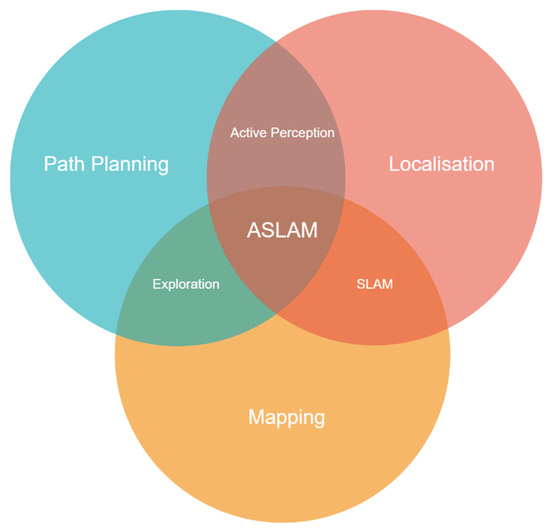
\includegraphics[width=0.5\linewidth]{../Localization/images/ASLAMDiagram.jpg}
		\caption{Active SLAM Venn Diagram \cite{Mihalik:2022}}
	\end{figure}
	
}

\STANDARD{Simultaneous Localization and Mapping}
{
	\begin{figure}
		\centering 
		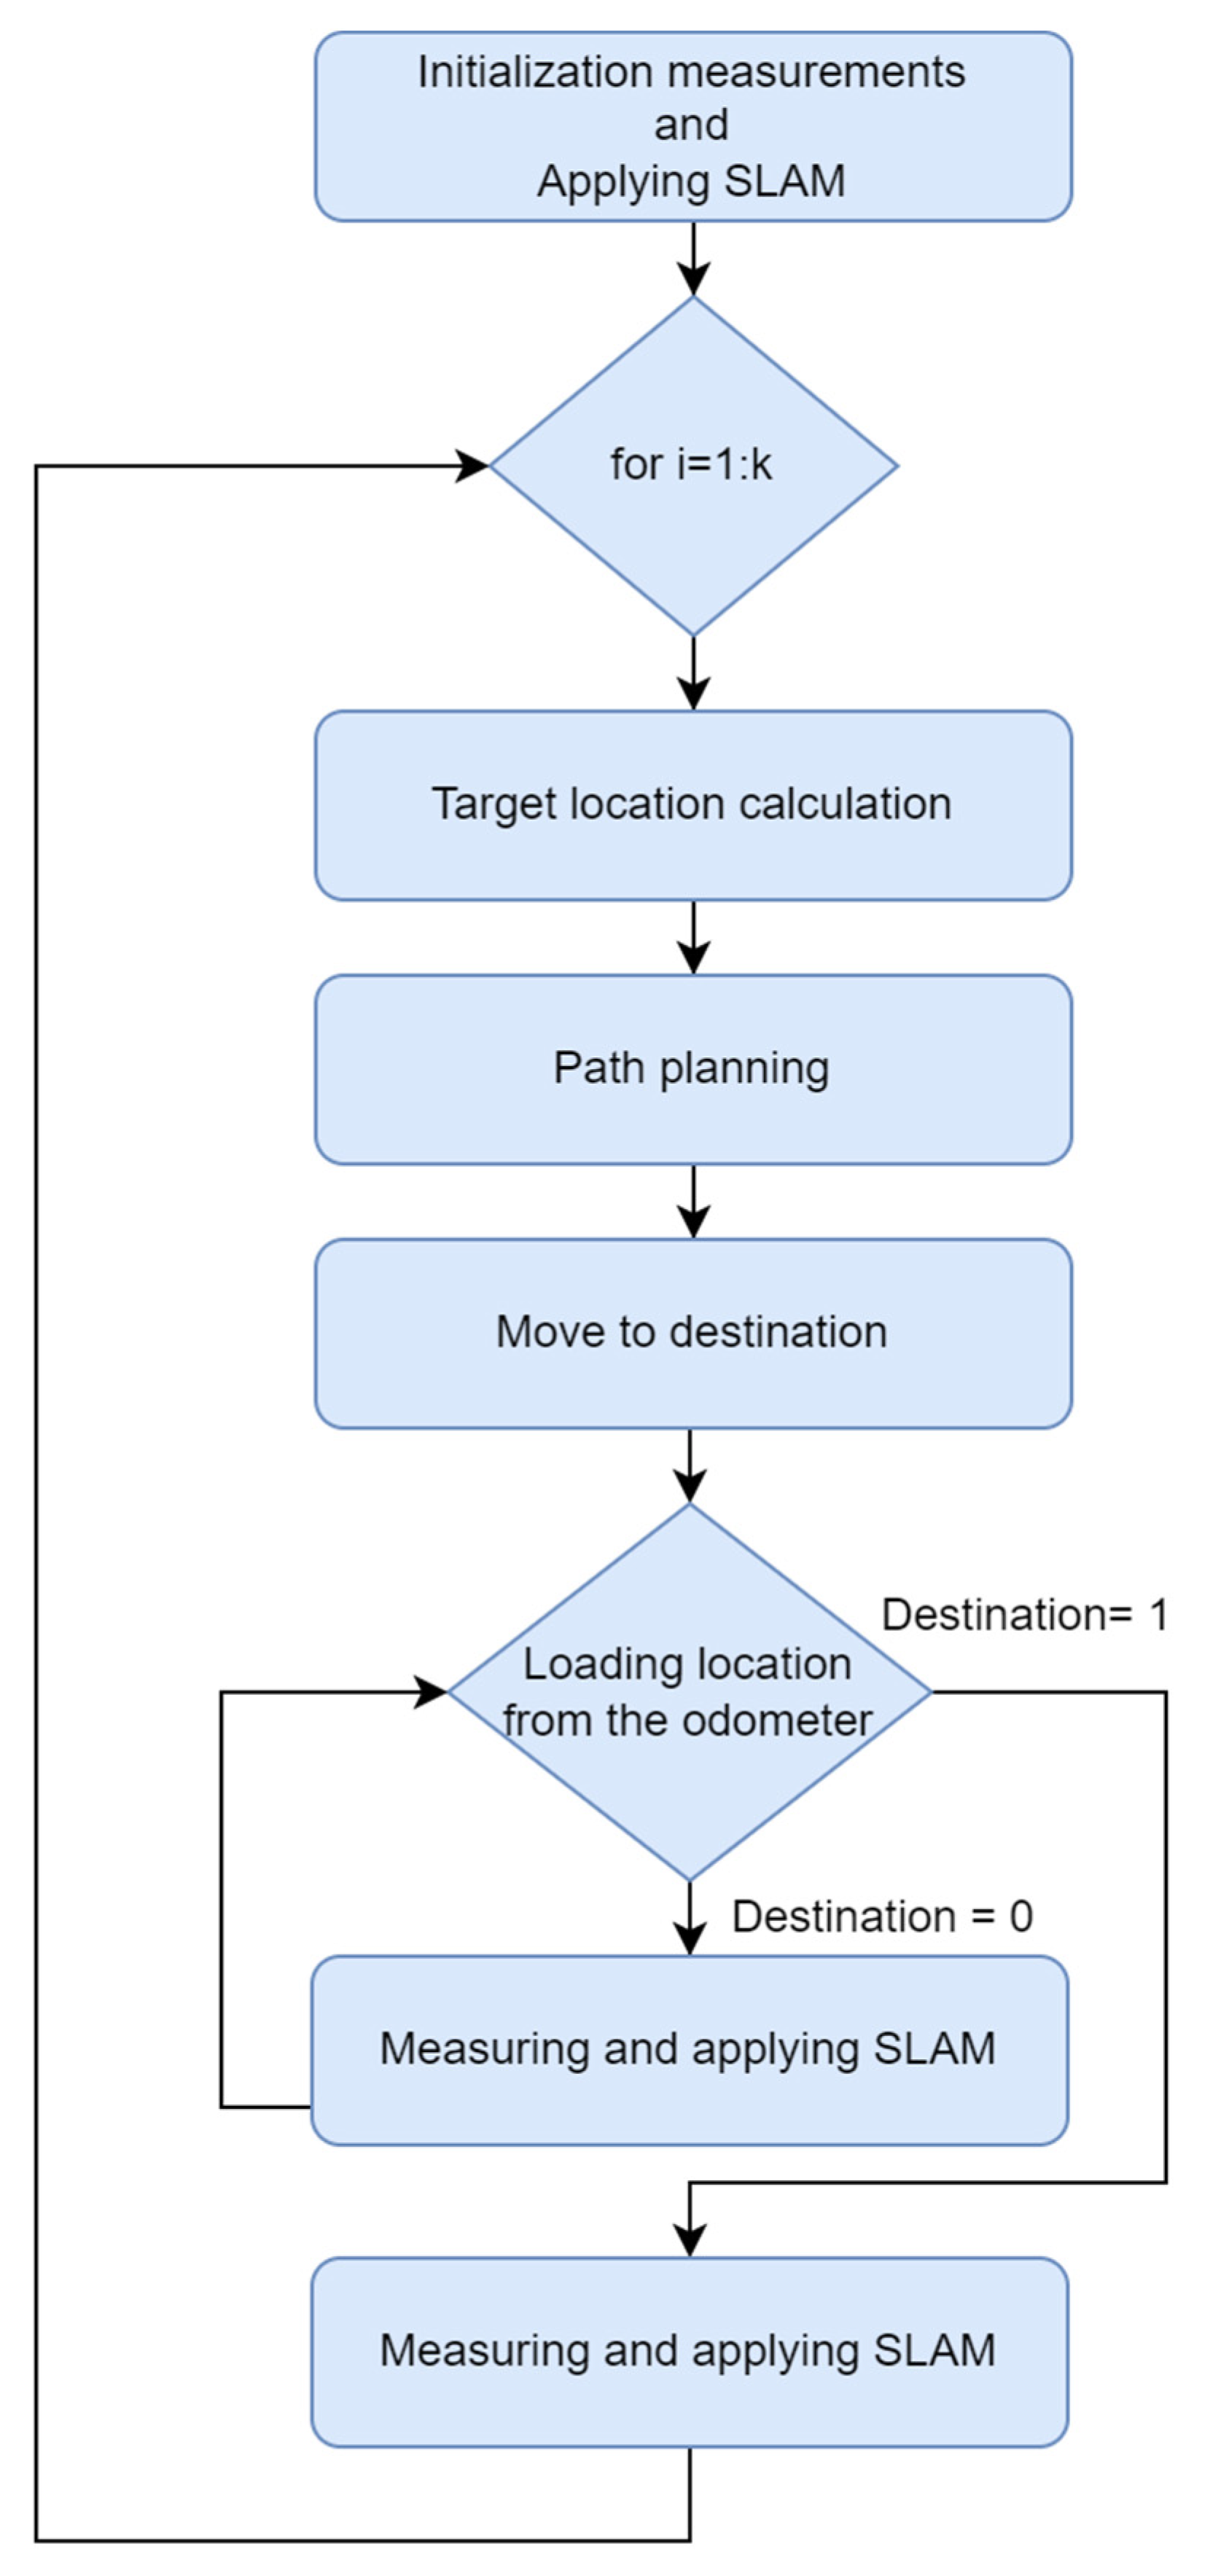
\includegraphics[width=0.25\linewidth]{../Localization/images/SLAMFlowchart.png}
		\caption{SLAM Flowchart \cite{Mihalik:2022}}
	\end{figure}

}

\Mysection{Multi-Agent and Distributed Localization}

\STANDARD{Distributed Localization for Multi-Robot Systems}{
	\textbf{Motivation}
	\begin{itemize}
		\item Necessary for swarms, collaborative tasks, and robust large-area coverage.
		\item Emphasizes resilience and scalability by avoiding centralized processing.
	\end{itemize}
	\vspace{0.3cm}
	\textbf{Distributed Relative Localization}
	\begin{itemize}
		\item Robots use \textbf{local information} (e.g., inter-robot distance/bearing) to estimate their own position and the positions of their neighbors.
		\item Algorithms must manage \textbf{communication latency} and \textbf{non-global consensus} for network coordination \cite{Wang:2023}.
	\end{itemize}
}

\Mysection{Deep Learning in Localization}
\STANDARD{Multi-Time Pressure and Eigenvector Feature(MTPEF)}
{
	\begin{figure}
		\centering 
		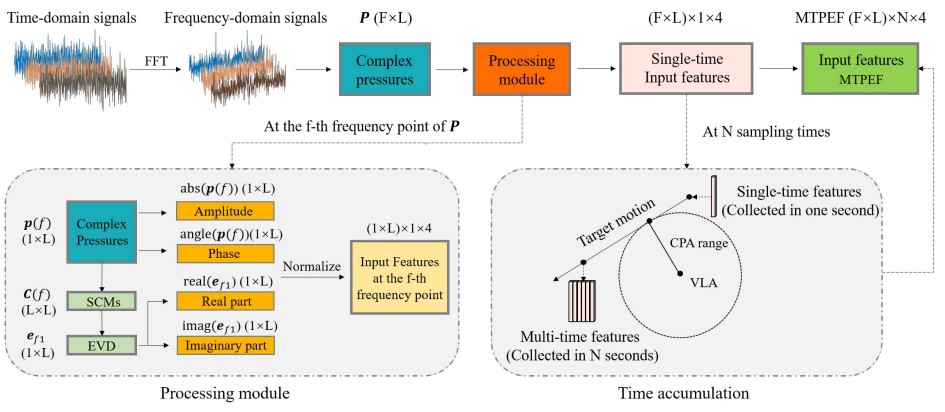
\includegraphics[width=\linewidth]{../Localization/images/MTPEF.jpg}
		\caption{Multi-Time Pressure and Eigenvector Feature \cite{Sun:2024}}
	\end{figure}
}
\STANDARD{Deep Learning for Localization and Mapping (DL-LM)}{
	\textbf{The Data-Driven Approach}
	\begin{itemize}
		\item Uses neural networks to \textbf{learn the localization function} directly from raw sensor data, offering robustness over hand-engineered models.
	\end{itemize}
	\vspace{0.3cm}
	\textbf{Applications}
	\begin{itemize}
		\item \textbf{Visual SLAM/Odometry:} Learning pose regression or feature extraction from camera data  \cite{Chen:2023}.
		\item \textbf{Acoustic Source Localization:} Using DNNs for direction of arrival (DoA) estimation in noisy environments \cite{Grumiaux:2022} and via improved input features  \cite{Sun:2024}.
		\item \textbf{Microscopy Localization:} Applying lightweight DL for precise localization of single molecules in high-resolution bioimaging  \cite{Fei:2025}.
	\end{itemize}
}     
\STANDARD{Network Structure: Inception and Residual}{
	\textbf{The IRSNet Architecture}
	\begin{itemize}
		\item \textbf{IRSNet} (Inception and Residual in-series Network) is the network structure designed specifically for the deep learning acoustic source localization method.
		\item \textbf{Inception Modules:} These are incorporated to effectively capture feature information at \textbf{multiple scales} from the MTPEF input features.
		\item \textbf{Residual Modules:} These are used to facilitate the training of a \textbf{deep network} by creating shortcut connections (skip connections) that help prevent the problem of gradient degradation and diminishing returns as the network depth increases.
		\item \textbf{Goal:} This tailored combination significantly \textbf{boosts localization accuracy} and robustness, especially for underwater acoustic characteristics.\cite{Sun:2024}
	\end{itemize}
}
\STANDARD{IRSNet Architecture}
{
	\begin{figure}
		\centering 
		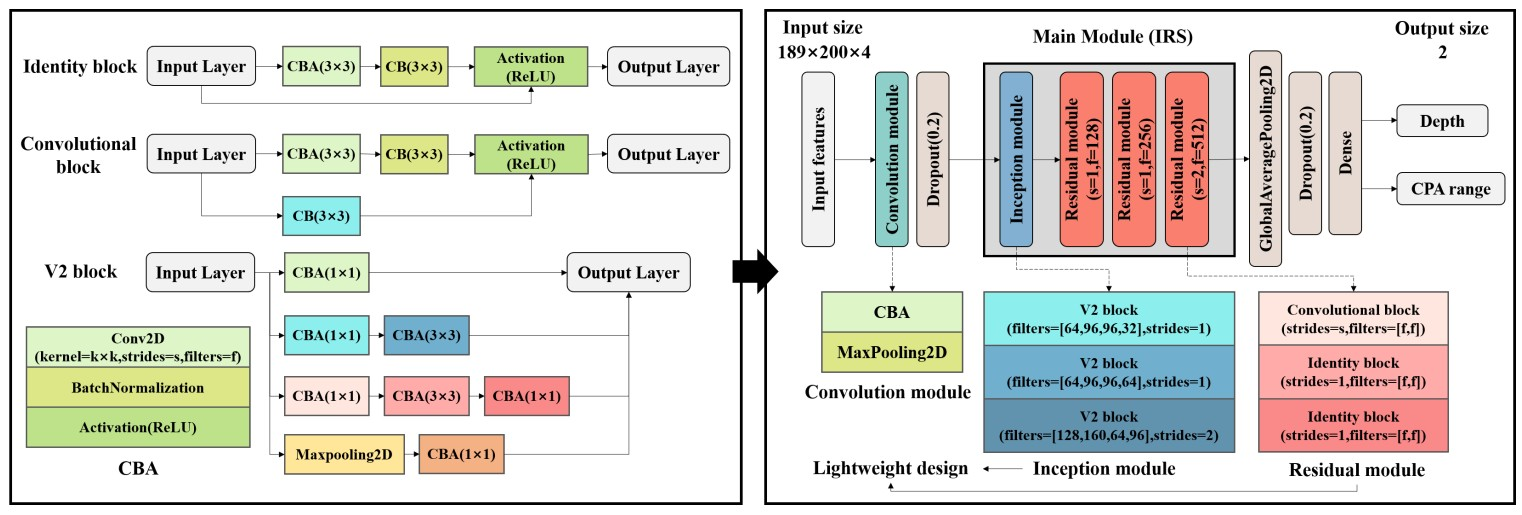
\includegraphics[width=\linewidth]{../Localization/images/IRSNetDN.jpg}
		\caption{Inception and Residual in-series Network \cite{Sun:2024}}
	\end{figure}
}
                                                                                                        